\documentclass[12pt, a4paper]{article}
\usepackage[utf8]{inputenc}
\usepackage{amsmath}
\usepackage{relsize}
\usepackage{array}
\usepackage{xcolor}
\usepackage{courier}
\usepackage{listings}
\lstset{basicstyle=\footnotesize\ttfamily,breaklines=true}
\lstset{framextopmargin=50pt,frame=bottomline}
\usepackage{tikz}
\usetikzlibrary{calc}
\usepackage{graphicx}
\graphicspath{ {./images/} }
\usepackage{multirow}

\begin{document}

\section*{Problem 1}
\subsection*{a.}

\begin{align*}
		(\lambda f . \lambda g . f(g\ 1) (\lambda x . x + 4)) (\lambda y . 3 - y)
		&= (\lambda g . (g\ 1) + 4) (\lambda y . 3 - y) \\
		&= (3 - 1) + 4 \\
		&= 6
\end{align*}

\subsection*{b.}
\begin{align*}
		(\lambda f . \lambda g . f(g\ 1) (\lambda x . x + 4)) (\lambda y . 3 - y)
		&= \lambda f . f(3 - 1) (\lambda x . x + 4) \\
		&= (3 - 1) + 4 \\
		&= 6
\end{align*}


\section*{Problem 2}
\begin{align*}
\begin{split}
	(\lambda \text{compose} . (\lambda h . \text{compose}\ h\ h\ 3)\ \lambda x . x + x) \\
\lambda f . \lambda g . \lambda x . f(g\ x) \\
	&= (\lambda \text{compose} . \\
	& \text{compose}\ (\lambda x . (x + x)\ (\lambda x . (x + x)\ 3)) \\
	& \lambda f . \lambda g . \lambda x . f(g\ x) \\
	&= (\lambda \text{compose} . \text{compose}\ 12)\ \lambda f . \lambda g . \lambda x . f(g\ x) \\
	&= \lambda f . (\lambda g . \lambda x . f(g\ x)\ 12) \\
	&= \lambda f . \lambda x . f(12 \ x)
\end{split}
\end{align*}

\section*{Problem 3}
\begin{align*}
	<s> &::=\ <c> | <d><s> | <s><d> \\
	<c> &::= 111 \\
	<d> &::= 0\ |\ 1
\end{align*}


\section*{Problem 4}
\subsection*{a.}
\begin{center}
	\begin{tikzpicture}
	\node(graphic)[label=below:{(1 6 /) (4 \~{}) +}]
	{
		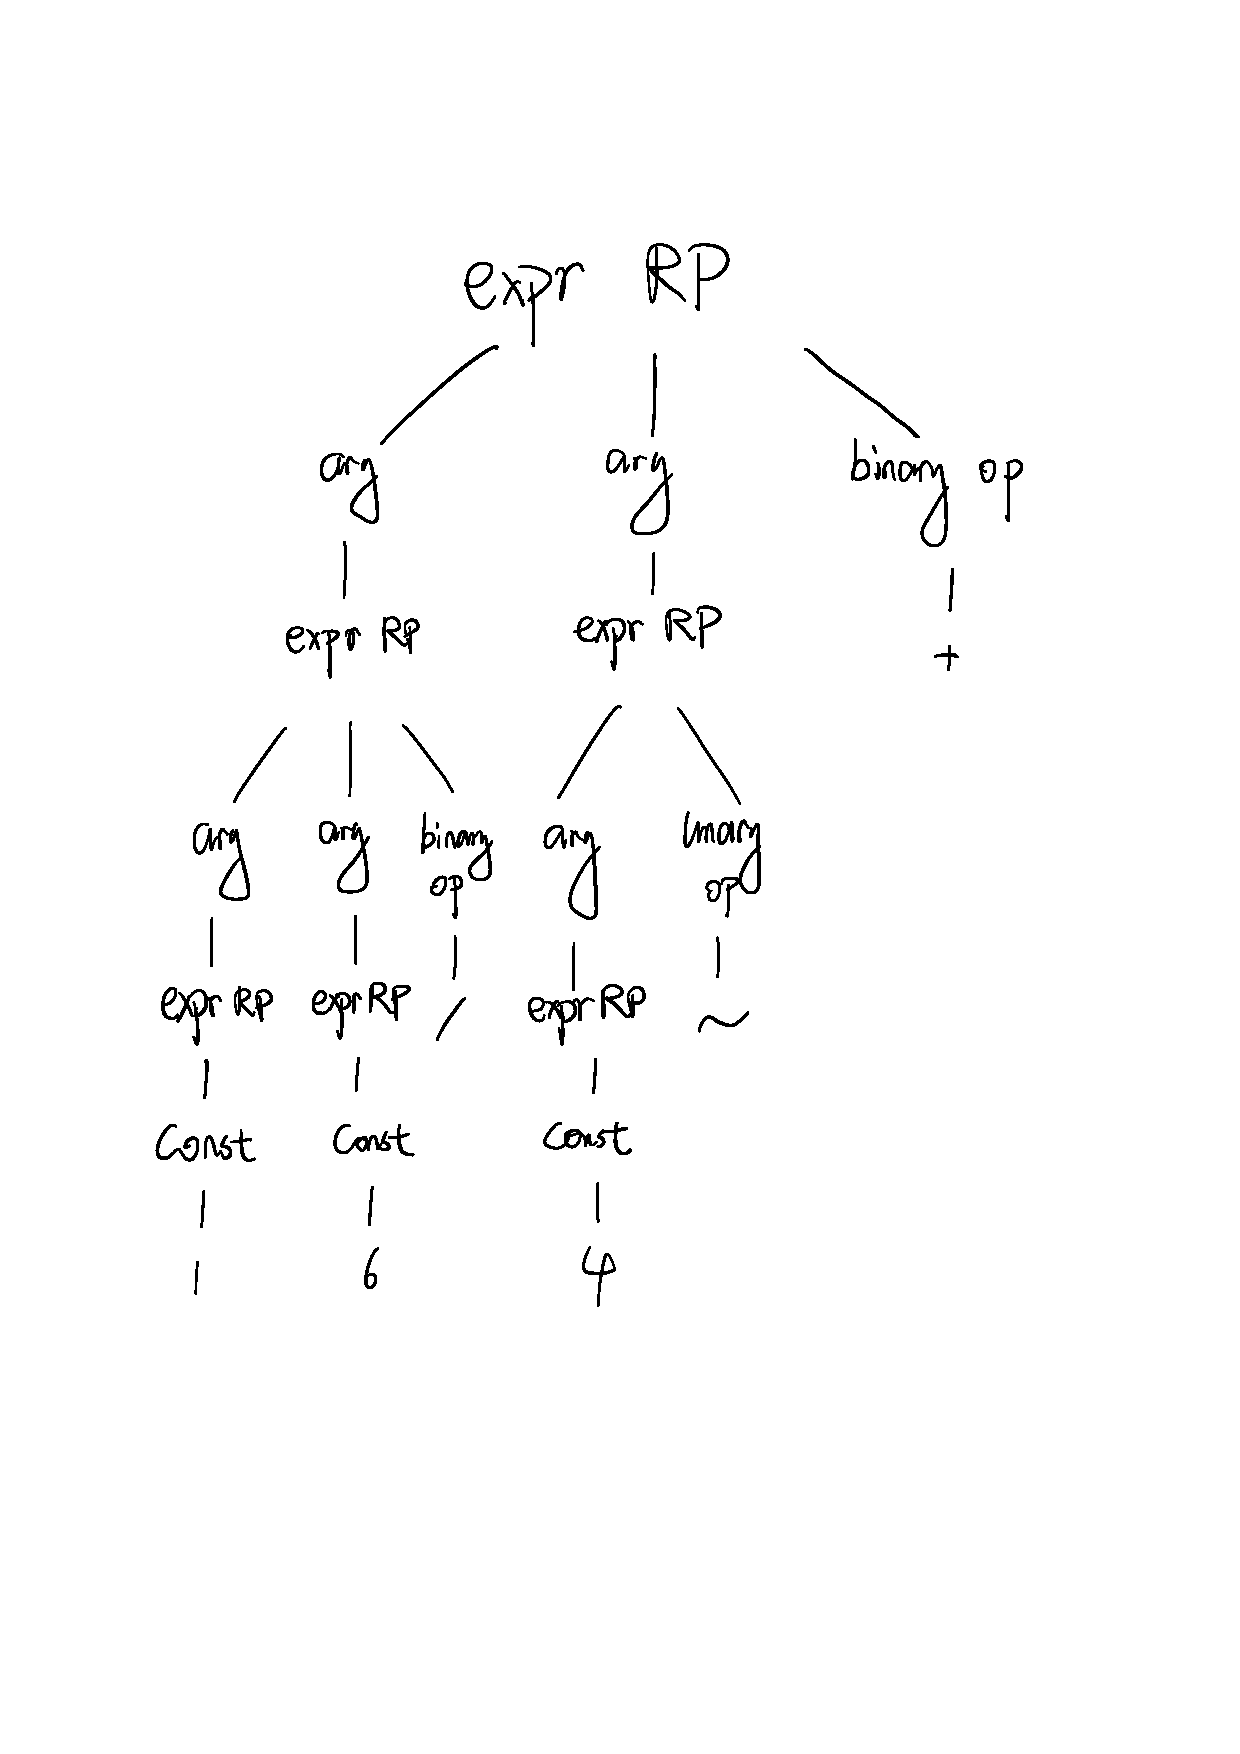
\includegraphics[scale=0.8]{Q4a.pdf}
	};
	\end{tikzpicture}
\end{center}

\subsection*{b.}
\begin{center}
	\begin{tikzpicture}
	\node(graphic)[label=below:{((8 \~{}) 7 +) 3 /}]
	{
		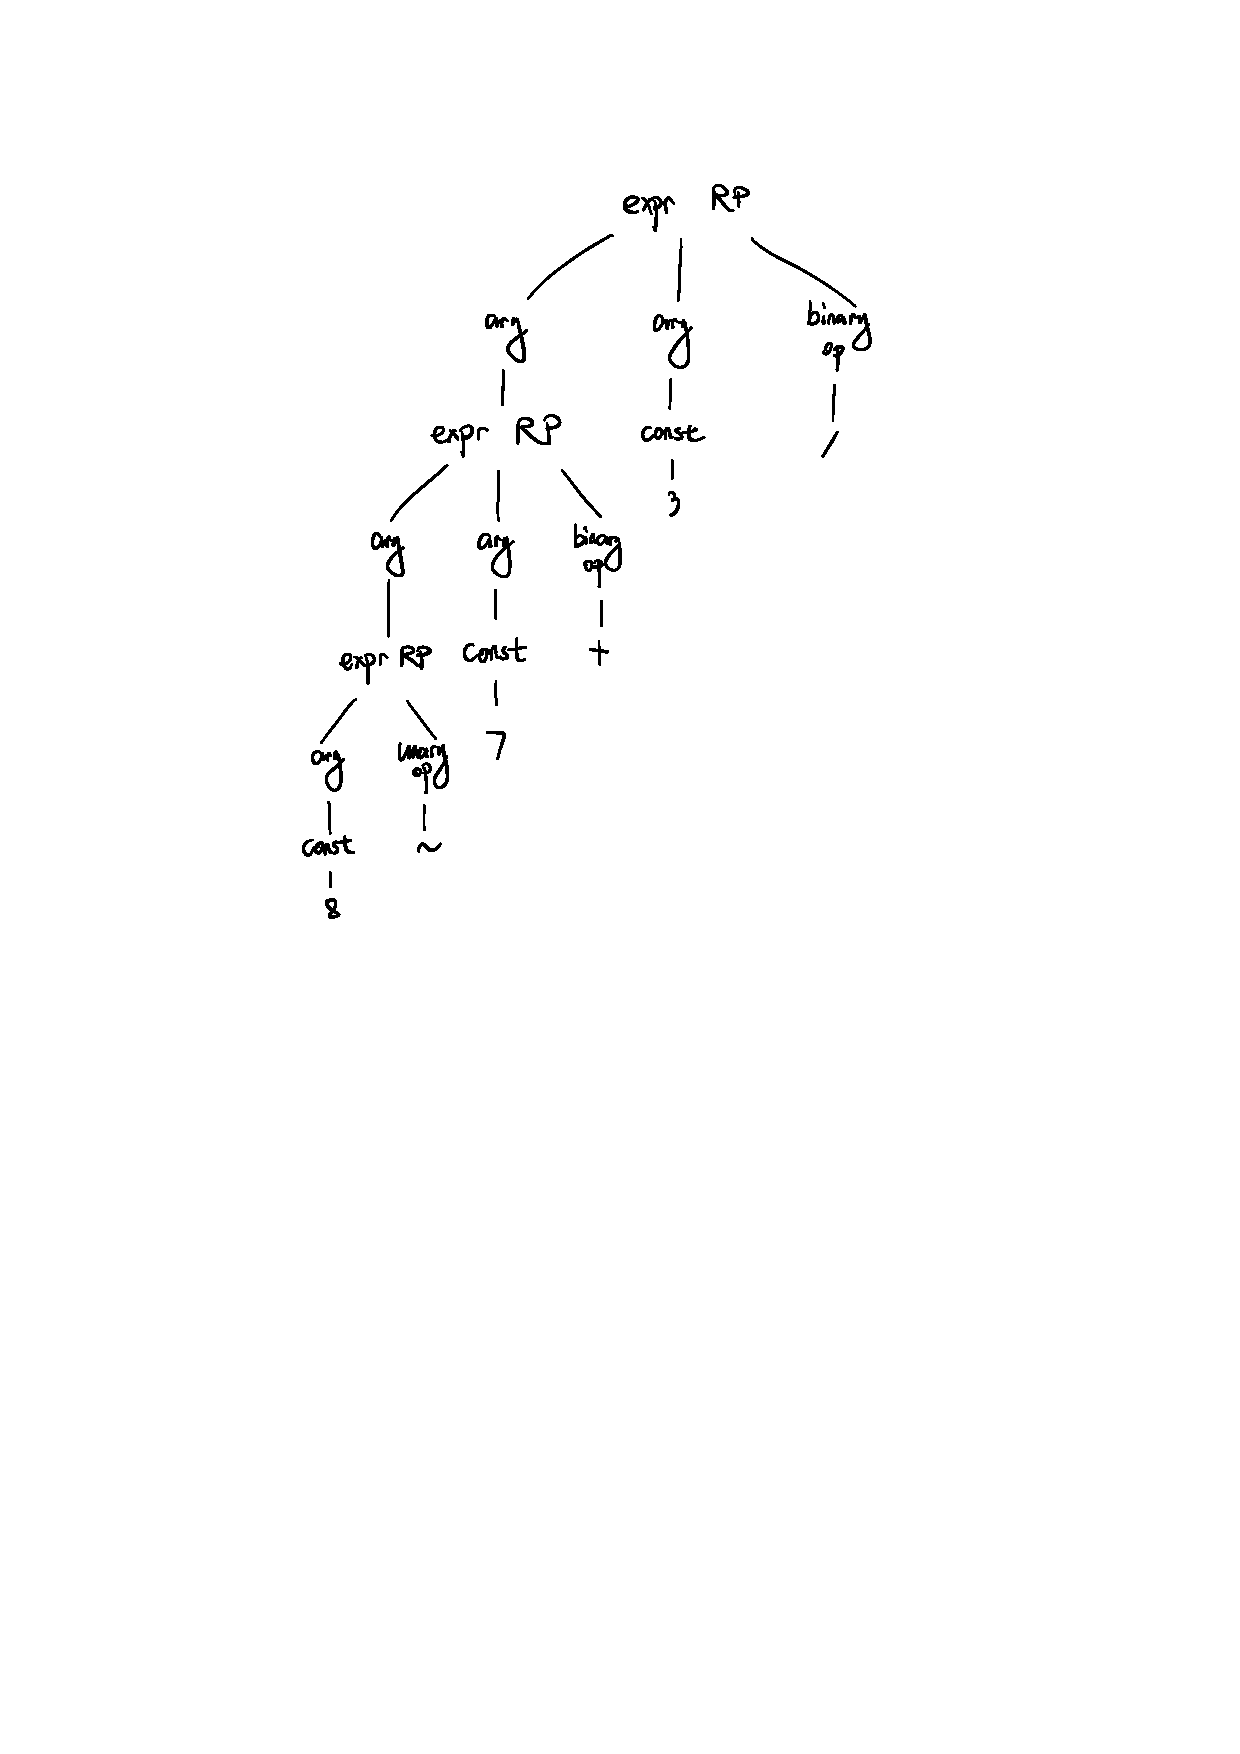
\includegraphics[scale=1.2]{Q4b.pdf}
	};
	\end{tikzpicture}
\end{center}

\section*{Problem 5}
For example, $a * b * c$ can be evaluated in following two ways:
$$(a * b) * c$$
$$a * (b * c)$$
Therefore the grammar is ambiguous.
Unambiguous grammar:
\begin{align*}
	<S> &::=\ <X> \\
	<X> &::=\ <X> * <Y>\ |\ <Y> \\
	<Y> &::= a\ b\ c
\end{align*}
\end{document}
